%!TEX root = ../var.tex

\subsection{Экспериментальное нахождение вероятности}

В этом пункте описан способ экспериментального определения вероятности
наступления так называемых массовых событий.

\begin{definition}
	\label{def:4.1}
  	Событие A называется \textit{массовым}, если опыт (эксперимент, испытание), при котором событие A может произойти, можно повторить \textit{неограниченное число раз при одних и тех же условиях}.
\end{definition} 

Методами теории вероятностей изучают (в основном) эксперименты, которые порождают массовые события. Всюду до конца лекций будут рассматриваться только массовые события.

\begin{example}
	\label{ex:4.2}
1) Опыт: однократное подбрасывание ломаного гроша.
События выпадение орла $O$ и выпадение решки $P$ являются массовыми событиями. Заметим, что пространство элементарных событий 
$\Omega = \{O, P \}$ состоит из конечного числа элементарных исходов.

2) Опыт: подбрасывание ломаного гроша до появления первого орла. События $P , OP , OOP, \ldots, O \ldots OP , \ldots$ являются массовым. Заметим, что в этом примере пространство $\Omega=\{P, OP, OOP, \ldots, O \ldots OP, \ldots\}$ состоит из
счётного количества элементарных исходов: положение кольца однозначно определяется положением его центра.

3) Опыт: бросание обручального кольца на клетчатую скатерть (диаметр кольца меньше стороны клетки). Событие $A$: кольцо падает внутрь какой-нибудь клетки, не пересекая её границы. Это событие является массовым.
Заметим, что в этом примере пространство состоит из несчётного количества элементарных исходов.
 \end{example} 

Типичность этих трёх примеров состоит в том, что в теории вероятностей встречаются три типа пространств элементарных событий: конечные, счётные и несчётные.

\begin{definition}
	\label{def:4.3}
	Если в результате n испытаний массовое событие $A$ произошло $\mu(A)$ раз, то число $\frac{\mu(A)}{n}$
называется \textit{относительной частотой} появления события $A$.
\end{definition}

Для каждого примера 4.2 можно провести $n$ опытов, сосчитать число $\mu(A)$ появлений этого события и подсчитать относительную частоту $\frac{\mu(A)}{n}$.

Массовые события обладают свойством <<статистической устойчивости>>, а именно: \textit{при увеличении числа экспериментов относительная частота $\frac{\mu(A)}{n}$
появления события $A$ имеет тенденцию стабилизироваться, стремясь к некоторому числу $\P(A)$.}
\begin{definition}
	\label{def:4.4}
Число $\P(A) = \lim\limits_{n\to\infty} \frac{\mu(A)}{n}$ называется \textit{статистической вероятностью} события $A$ и находится при больших $n$ по приближённой формуле $\P(A)\approx \mu(A)$.
\end{definition} 

\subsection{Вероятность на конечном пространстве.}
Пусть задано конечное пространство $\Omega=\{\omega_1,\omega_2,\ldots,\omega_n\}$, состоящее из $n$ элементарных событий (исходов), и заданы вероятности наступления этих
событий $\P(\omega_1 ) = p_1 , \P(\omega_2 ) = p_2 , \ldots , \P(\omega_n ) = p_n$ так, что $p_1 + p_2 + \ldots + p_n = 1$.
Обозначим через $\omega$ переменную величину, принимающую значения из $\Omega$.

\begin{definition}
	\label{def:4.5}
Такое соответствие записывается в виде таблицы
\begin{center}
	\begin{tabular}{|l|l|l|l|l|}
		\hline
		$\omega$ & $\omega_1$ & $\omega_2$ & $\ldots$ & $\omega_n$ \\ \hline
		$\P(\xi)$  & $p_1$ & $p_2$ & $\ldots$  & $p_n$ \\ \hline
	\end{tabular}
\end{center}


которая называется \textit{рядом распределения} случайных исходов или \textit{законом
распределения}. Если $n = 2$, то ряд называется \textit{схемой Бернулли}. Если $n \geq 3$,
то ряд называется \textit{схемой независимых испытаний с несколькими исходами}.
\end{definition}

Ряд распределения задаёт функцию в виде таблицы, которая каждому элементарному исходу ставит в соответствие вероятность его наступления.

Потребуем теперь выполнение аксиомы $\mathcal{P}3$.

\begin{deflemma}[Формула вероятности на конечном пространстве]
	\label{def:4.6}
Если  вероятность, определяемая рядом распределения из опред. 4.5, подчиняется аксиоме $\mathcal{P}3$, то вероятность события $A = \{\omega_{i_1} , \omega_{i_2} , \ldots ,  \omega_{i_k} \} \subset \Omega$ вычисляется по формуле
%
$$\P(A) = p_{i_1} + p_{i_2} + \ldots + p_{i_k} ,$$

которая называется формулой вероятности на конечном пространстве.
\end{deflemma}
\begin{proof}
\begin{gather*}
 	\P(A) = \P (\omega_{i_1} , \omega_{i_2} , \ldots , \omega_{i_k}) =\\= \P \left( \bigcup\limits_{j=1}^k \{\omega_{i_j} \} \right) \stackrel{\mathcal{P}3}{=} \sum_{j=1}^{k} \P(\omega_{i_j}) = \sum_{j=1}^{k} p_{i_j} = p_{i_1} + p_{i_2} + \ldots + p_{i_k}.
\end{gather*}
\end{proof} 
\begin{example}
	\label{ex:4.7}
Простейший ряд распределения имеет эксперимент с детерминированным исходом, $\Omega = \{ \omega \}$ (см. опред. \ref{def:2.3}):
\begin{center}
	\begin{tabular}{|l|l|}
		\hline
		$\xi$ & $\omega$  \\ \hline
		$\P$  & $1$  \\ \hline
	\end{tabular}
\end{center}
Этот тривиальный случай удовлетворяет всем аксиомам и определениям, однако никакого значения в теории вероятностей не имеет. Придётся с этим
мириться.
\end{example}
\begin{definition}
	\label{def:4.8}
	Пусть в результате опыта могут возникнуть только
два события: <<успех>>, который обозначается единицей — 1 и наступает c вероятностью $p$, и <<неудача>>, которая обозначается нулём — 0 и наступает c
вероятностью $q = 1−p$; $\Omega = \{0, 1\}$. Такой опыт называется \textit{схемой Бернулли}\footnote{
	Якоб Бернулли (Jakob Bernoulli, 1654-1705), швейцарский математик
}
и имеет ряд распределения

\begin{center}
	\begin{tabular}{|c|c|c|}
		\hline
		$\xi$ & 0 & 1  \\ \hline
		$\P$  & $q=1-p$ & p \\ \hline
	\end{tabular}
\end{center}

\end{definition}

Схема Бернулли является первым нетривиальным примером вероятности на конечном пространстве.

Схема Бернулли имеет простую интерпретацию. Рассмотрим ломаный грош с вероятностями выпадения орла $p$ и решки $q = 1 − p$. Обозначим появление орла через 1, а его не выпадение через 0, получим схему Бернулли.

\begin{example}[Геометрическая интерпретация схемы независимых  испытаний с несколькими исходами]
	\label{ex:4.9}
Рассмотрим произвольный выпуклый многогранника с $n$ гранями, на которых написаны символы $\omega_1 , \omega_2 , \ldots , \omega_n$.

При этом многогранник должен быть таким, чтобы перпендикуляр, опущенный из его центра тяжести на любую грань, пересекал эту грань в её внутренней точке (чтобы многогранник, падая на эту грань, не перекатывался на другую).

Пусть вероятности выпадения многогранника гранью вниз равны соответственно $p_1 , p_2 , \ldots , p_n$ , где естественно $p_1 + p_2 + \ldots +p_n = 1$. 

Легко видеть, что вероятность $p_i$ пропорциональна телесному углу $\alpha_i$ с вершиной $C$ в центре тяжести многогранника, опирающегося на грань $\omega_i$.

Так как сумма всех телесных углов с вершиной $C$ равна $4\pi$ стерадиан, т.е. $\alpha_1 + \alpha_2 + \ldots + \alpha_n = 4\pi$, то
$$\frac{\alpha_1}{4\pi} + \frac{\alpha_2}{4\pi} + \ldots + \frac{\alpha_n}{4\pi}
 = 1,$$ поэтому $p_i = 4\pi$.
\end{example}

\subsection{Классическая вероятность}

Классическая вероятность является частным случаем вероятности на конечном пространстве, когда вероятность подчинена принципу равной вероятности. Исторически классическая вероятность применялась в теории азартных игр и появилась раньше вероятности на конечном пространстве.

\textbf{Принцип равной вероятности.} \textit{Если на конечном пространстве $\Omega$ вероятность наступления его элементарных исходов $\omega_1 , \omega_2 , \ldots , \omega_n$ одна и та же,
$$p_1 = p_2 = \ldots = p_n = p,$$
то говорят, что вероятность на конечном пространстве удовлетворяет
принципу равной вероятности (или равной возможности).}

Выпадение орла и решки при подбрасывании симметричной монеты; выпадение граней при подбрасывании правильного многогранника (тетраэдра, куба, октаэдра, додекаэдра или икосаэдра); появление к.-л. карты из полной
колоды карт удовлетворяют принципу равной возможности.

Классическая вероятность характеризуется только числом элементарных исходов $n$ в пространстве $\Omega$. Она имеет ряд распределения

\begin{center}
	\begin{tabular}{|c|c|c|c|c|}
		\hline
		$\omega$ & $\omega_1$ & $\omega_2$ & $\ldots$ & $\omega_n$ \\ \hline
		$\P(\omega)$  & $p$ & $p$ & $\ldots$  & $p$ \\ \hline
	\end{tabular}
\end{center}

где $np = 1$, поэтому $p = \frac{1}{n}$.


\begin{lemma}[Формула классической вероятности]
	\label{lemma:4.10}
Если вероятность $\P$ удовлетворяет принципу равной возможности, то вероятность наступления события $A = \{ \omega_{i_1} , \omega_{i_2} , \ldots , \omega_{i_k} \} \subset \Omega$ определяется по формуле, называемой формулой классической вероятности,
$$\P(A) = \frac{k}{n}$$
\end{lemma} 
\begin{proof}
	$\P(A) = p_{i_1} + p_{i_2} + \ldots + p_{i_k} = kp = \frac{k}{n}$
\end{proof}

Если обозначить число $k$ элементов множества $A$ через $\mu(A)$, а число $n$ элементов пространства $\Omega$ через $\mu(\Omega)$, то формулу классической вероятности
можно записать в виде
$$\P(A) = \frac{\mu(A)}{\mu(\Omega)}$$
Число $\mu(A) = k$ называется числом исходов, \textit{благоприятствующих} наступлению события $A$.

\begin{zam}
	\label{zam:4.11}
1) Вероятности элементарных исходов в экспериментах с шариками, описанные в теоремах \ref{th:1.4}, \ref{th:1.6} и \ref{th:1.7}, удовлетворяют принципу равной возможности. Эти вероятности соответственно $1/A_n^k , 1/C_n^k$ и $1/n^k$.

2) Вероятности элементарных исходов в теореме \ref{th:1.9} (выбор с возвращением и без учёта порядка) не удовлетворяют этому принципу. Например, при $n = 2$
и $k = 2$ вероятности элементарных событий имеют ряд распределения

\begin{center}
	\begin{tabular}{|c|c|c|c|}
		\hline
		$\omega$ & $(1,1)$ & $(1,2)$ & $(2,2)$ \\ \hline
		$\P(\omega)$  & $1/4$ & $1/2$  & $1/4$ \\ \hline
	\end{tabular}
\end{center}

3) Следует отметить, что при рассмотрении подобных вопросов ошибались даже такие великие математики, как, например, Д'Аламбер. 

Так, однажды у Даламбера спросили, с какой вероятностью монета, брошенная дважды, хотя бы один раз выпадет гербом. Ответ учёного был $\frac{2}{3}$, т.к. он считал, что есть 3 возможных исхода (герб-герб, герб-решка, решка-решка) и среди них 2 благоприятствующих. 

Д'Аламбер пренебрегал тем, что эти три возможных исхода не равновозможны. 

Правильным ответом является $\frac{3}{4}$ , поскольку из четырёх равновозможных исходов (герб-герб, герб-решка, решка-герб, решка-решка) три благоприятствуют указанному событию. 

Точка зрения Д'Аламбера была даже опубликована во Французской энциклопедии в 1754 г. в статье <<Герб и решётка>> (<<Croix on pile>>).
\end{zam}
 

\subsection{Вероятность на счётном пространстве}
Пусть теперь $\Omega = \{\omega_1 , \omega_2 , \ldots , \omega_n , \ldots \}$ – счётное пространство. Пусть $p_1 + p_2 + \ldots + p_n + \ldots = 1$ — сходящийся (к единице) числовой ряд, удовлетворяющий
для всех $i \in \mathbb{N}$ условию $0 < p_i < 1$. Последнее условие позволяет трактовать члены этого ряда как вероятности элементарных событий пространства $\Omega$.

\begin{definition}
	\label{def:4.12}
Вероятность элементарных исходов, заданная в виде таблицы
\begin{center}
	\begin{tabular}{|c|c|c|c|c|c|}
		\hline
		$\omega$ & $\omega_1$ & $\omega_2$ & $\ldots$ & $\omega_i$ & $\ldots$ \\ \hline
		$\P(\omega)$  & $p_1$ & $p_2$ & $\ldots$  & $p_i$ & $\ldots$ \\ \hline
	\end{tabular}
\end{center}
называется \textit{рядом распределения на счётном пространстве}.
Потребуем теперь выполнение аксиомы $\mathcal{P}3$.
\end{definition}

\begin{lemma}[Формула вероятности на счётном пространстве]
	\label{lemma:4.13}
Если события из пространства $\Omega$ подчиняются аксиоме $\mathcal{P}3$, то вероятность события $A = \{\omega_{i_1} , \omega_{i_2} , \ldots , \omega_{i_k} , \ldots \} \subset \Omega$ вычисляется по формуле
$$\P (A) = p_{i_1} + p_{i_2} + \ldots + p_{i_k} + \ldots$$
\end{lemma}

\begin{proof}
\begin{gather*}
	\P(A) = \P(\omega_{i_1},\omega_{i_2}, \ldots, \omega_{i_k}, \ldots) =\\= \P \left( \bigcup_{j=1}^\infty \{ \omega_{i_j}\} \right) \stackrel{\mathcal{P}3}{=} \sum_{j=1}^{\infty} \P(\omega_{i_j}) = \sum_{j=1}^{\infty} p_{i_j} = p_{i_1} + p_{i_2} + \ldots + p_{i_k} + \ldots 
\end{gather*}
	
\end{proof}

\begin{zam}
	\label{zam:4.14}
Каждому степенному ряду на той части его интервала
сходимости, на которой его члены положительны, можно поставить в соответствие параметрическое семейство распределений со счётным пространством.
Рассмотрим, например, экспоненту $e^\lambda$ . Её ряд МакЛорена
$$1+ \frac{\lambda}{1!} + \frac{\lambda^2}{2!} + \ldots + \frac{\lambda^k}{k!} + \ldots = e^\lambda$$
сходится при всех значениях $−\infty < \lambda < \infty$ и имеет положительные члены при $\lambda > 0$. Умножим обе части этого тождества на $e^{−\lambda}$ , получим тождество

$$e^{−\lambda}+ \frac{\lambda}{1!} e^{−\lambda} + \frac{\lambda^2}{2!} e^{−\lambda}+ \ldots + \frac{\lambda^k}{k!} e^{−\lambda} + \ldots= 1$$

Составим следующий ряд распределения:

\begin{center}
	\begin{tabular}{|c|c|c|c|c|c|c|}
		\hline
		$k$ 			& 0 								& 1 				  & 2 & $\ldots$ & $k$ 		& $\ldots$ \\ \hline
		&&&&&& \\[-1em] 
		$P_\lambda(k)$  & $e^{-\lambda}$ & $\frac{\lambda}{1!}e^{-\lambda}$ & $\frac{\lambda^2}{2!}e^{-\lambda}$ & $\ldots$ & $\frac{\lambda^k}{k!}e^{-\lambda}$& $\ldots$ \\[1ex] \hline
	\end{tabular}
\end{center}
\end{zam}

\begin{definition}
	\label{def:4.15}
Распределение, реализуемое этим рядом, называется \textit{распределением Пуассона с параметром $\lambda$.}

На рис. 25 показаны функции $P_\lambda (k)$ для для параметра $\lambda = 0, 1; 1; 10,$ где
пунктиром показаны огибающие. В каждом случае сумма длин вертикальных отрезков равна 1.

Распределение Пуассона описывает, например, вероятность $P_\lambda (k) = \frac{\lambda^k e^{-\lambda}}{k!}$
поступления на телефонную станцию $k$ звонков за какой-нибудь фиксированный промежуток времени, где число звонков $k = 0, 1, 2, \ldots$.
\end{definition}. 
\begin{zam}
	\label{zam:4.16}
Другим источником построения распределений со счётным пространством являются сходящиеся числовые ряды с положительными членами. Например, известно (Л. Эйлер), что
$$\frac{1}{1^2} + \frac{1}{2^2} + \frac{1}{3^2} + \ldots + \frac{1}{k^2} + \ldots = \frac{\pi^2}{6}.$$
Разделив обе части этого числового тождества на $\frac{\pi^2}{6}$ , можно получить (безымянный) ряд распределения, задаваемый формулой $\P(k) = \frac{1}{k^2} \cdot \frac{6}{\pi^2} = \frac{6}{\pi^2 k^2}$ , со счётным пространством $\Omega = \mathbb{N}$.
Среди числовых рядов наиболее встречающимися в теории вероятностей являются геометрические прогрессии с положительными членами.
\end{zam}

\begin{definition}
	\label{def:4.17}
Если члены ряда $p_1 + p_2 + \ldots + p_n + \ldots = 1$ положительны и являются членами убывающей геометрической прогрессией с первым членом $p_1 = p$ и с знаменателем $q = 1 − p$, то вероятность на счётном пространстве называется \textit{геометрическим распределением}. Геометрическое распределение имеет ряд
\begin{center}
	\begin{tabular}{|c|c|c|c|c|c|}
		\hline
		$\tau_1$ & $\omega_1$ & $\omega_2$ & $\ldots$ & $\omega_k$ & $\ldots$ \\ \hline
		$\P$  & $q$ & $qp$ & $\ldots$  & $q^{k-1}p$& $\ldots$ \\ \hline
	\end{tabular}
\end{center}
\end{definition}

\begin{example}
	\label{ex:4.18}

Рассмотрим схему Бернулли (ломаного гроша) с вероятностью <<успеха>> (выпадения орла -- события 1) равной $p$. Она имеет ряд распределения

\begin{center}
	\begin{tabular}{|c|c|c|}
		\hline
		$\xi$ & 0 & 1  \\ \hline
		$\P$  & $1-p$ & p \\ \hline
	\end{tabular}
\end{center}

Пусть эксперимент состоит в том, что испытания по схеме Бернулли проводятся неограниченное число раз. С таким экспериментом связаны две случайные величины: $\tau_1$ — номер первого выпавшего орла и $\tau_0$ — число выпавших решек, появившихся до первого орла. Легко подсчитать, что случайные величины $\tau_0$ и $\tau_1$ имеют ряды распределения

\begin{center}
	\begin{tabular}{|c|c|c|c|c|c|}
		\hline
		$\tau_0$ & $0$ & $1$ & $\ldots$ & $k$ & $\ldots$ \\ \hline
		$\P$  & $q$ & $qp$ & $\ldots$  & $q^k p$& $\ldots$ \\ \hline
	\end{tabular}
	\quad и \quad
	\begin{tabular}{|c|c|c|c|c|c|}
		\hline
		$\tau_1$ & $1$ & $2$ & $\ldots$ & $k$ & $\ldots$ \\ \hline
		$\P$  & $q$ & $qp$ & $\ldots$  & $q^{k-1} p$& $\ldots$ \\ \hline
	\end{tabular}
\end{center}

В строке вероятностей эти ряды содержат одну и ту же геометрическую
прогрессию; они называются соответственно $\tau_0$-- и $\tau_1$-- геометрическим распределениями. Эти случайные величины связаны очевидной формулой $\tau_1 = \tau_0 + 1$.

Формула вероятности для $\tau_0$ -- геометрического распределения определена по формуле
$$\P(\tau_0 = k) = q^k p,$$
где $0 < p < 1$ и $q = p − 1$.
Формула вероятности для $\tau_1$ -- геометрического распределения:
$$\P(\tau_1 = k) = q^{k−1} p,$$
где $0 < p < 1$ и $q = p − 1.$
\end{example}

\subsection{Геометрическая вероятность}

Рассмотрим ограниченную измеримую область $\Omega \subset \mathbb{R}^n$ , состоящую из несчётного множества точек. '

Измеримость области означает: на прямой область $\Omega \subset \mathbb{R}^1$ имеет конечную ненулевую длину, на плоскости область $\Omega \subset \mathbb{R}^2$ имеет конечную ненулевую площадь, в пространстве область $\Omega \subset \mathbb{R}^3$ имеет конечный ненулевой объём и т.д. 

Пусть на $\Omega$ определена $\sigma$-алгебра $\mathfrak{A}$. Для любого события $A \in \mathfrak{A}$ обозначим через $\mu(A)$ его меру (длину, площадь, объём и т.д. соответственно). 

Пусть эксперимент состоит в том, что в область $\Omega$ бросают точку.

\textbf{Принцип равномерности}\footnote{
Вероятности, которые не подчиняются этому принципу, являются главным предметом изучения теории вероятностей. Они будут изучены в гл. 2. <<Теория случайных величин>>.	
}. 
\textit{Если для любого события $A \in \mathfrak{A}$ его вероятность задаётся по формуле
$$\P(A) = \alpha \mu(A),$$
где $\alpha$ — постоянное число, независящее от выбора события $A$ (т.е. не зависящее от формы $A$ и его расположения в $\Omega$), то говорят, что вероятность $\P(A)$ удовлетворяет принципу равномерности.}

\begin{lemma}
	\label{lemma:4.19}
Если вероятность $\P(A)$ удовлетворяет принципу равномерности, то
$$\alpha=\frac{1}{\mu(\Omega)}$$
\end{lemma}

\begin{proof}
	Подставим в формулу $\P(A) = \alpha \mu(A)$ достоверное событие $\Omega \in \mathfrak{A}$, получим: $1 = \alpha\mu(\Omega).$
\end{proof} 

\begin{definition}
	\label{def:4.20}
Полученная формула
$$\P(A) = \frac{\mu(A)}{\mu(\Omega)}$$
называется формулой \textit{геометрической} вероятности. (Не путать с геометрическим рядом распределения!)
\end{definition}

\begin{figure}[H]
	\centering
	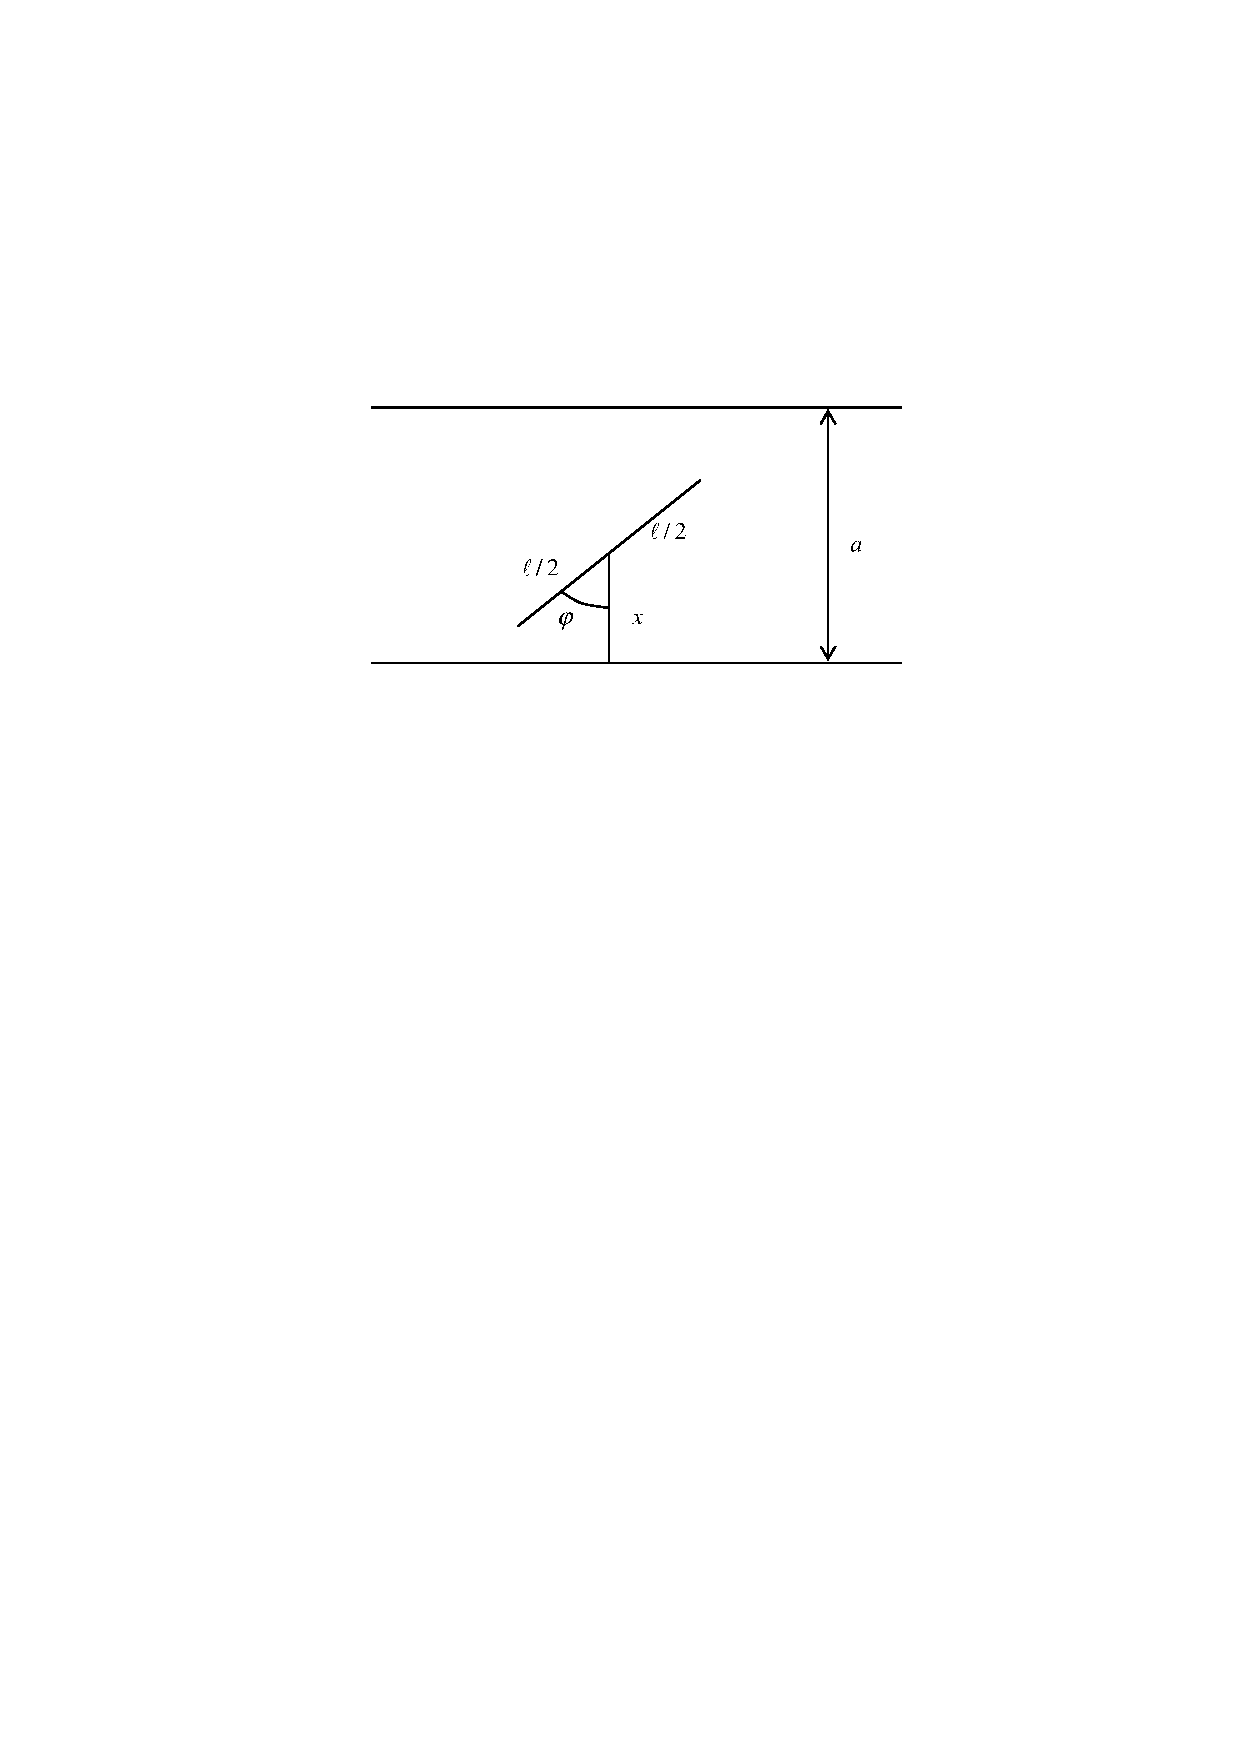
\includegraphics[]{pic/pic3}
	\caption{Задача Бюффона}
	\label{fig3}
\end{figure}
\begin{figure}[H]
	\centering
	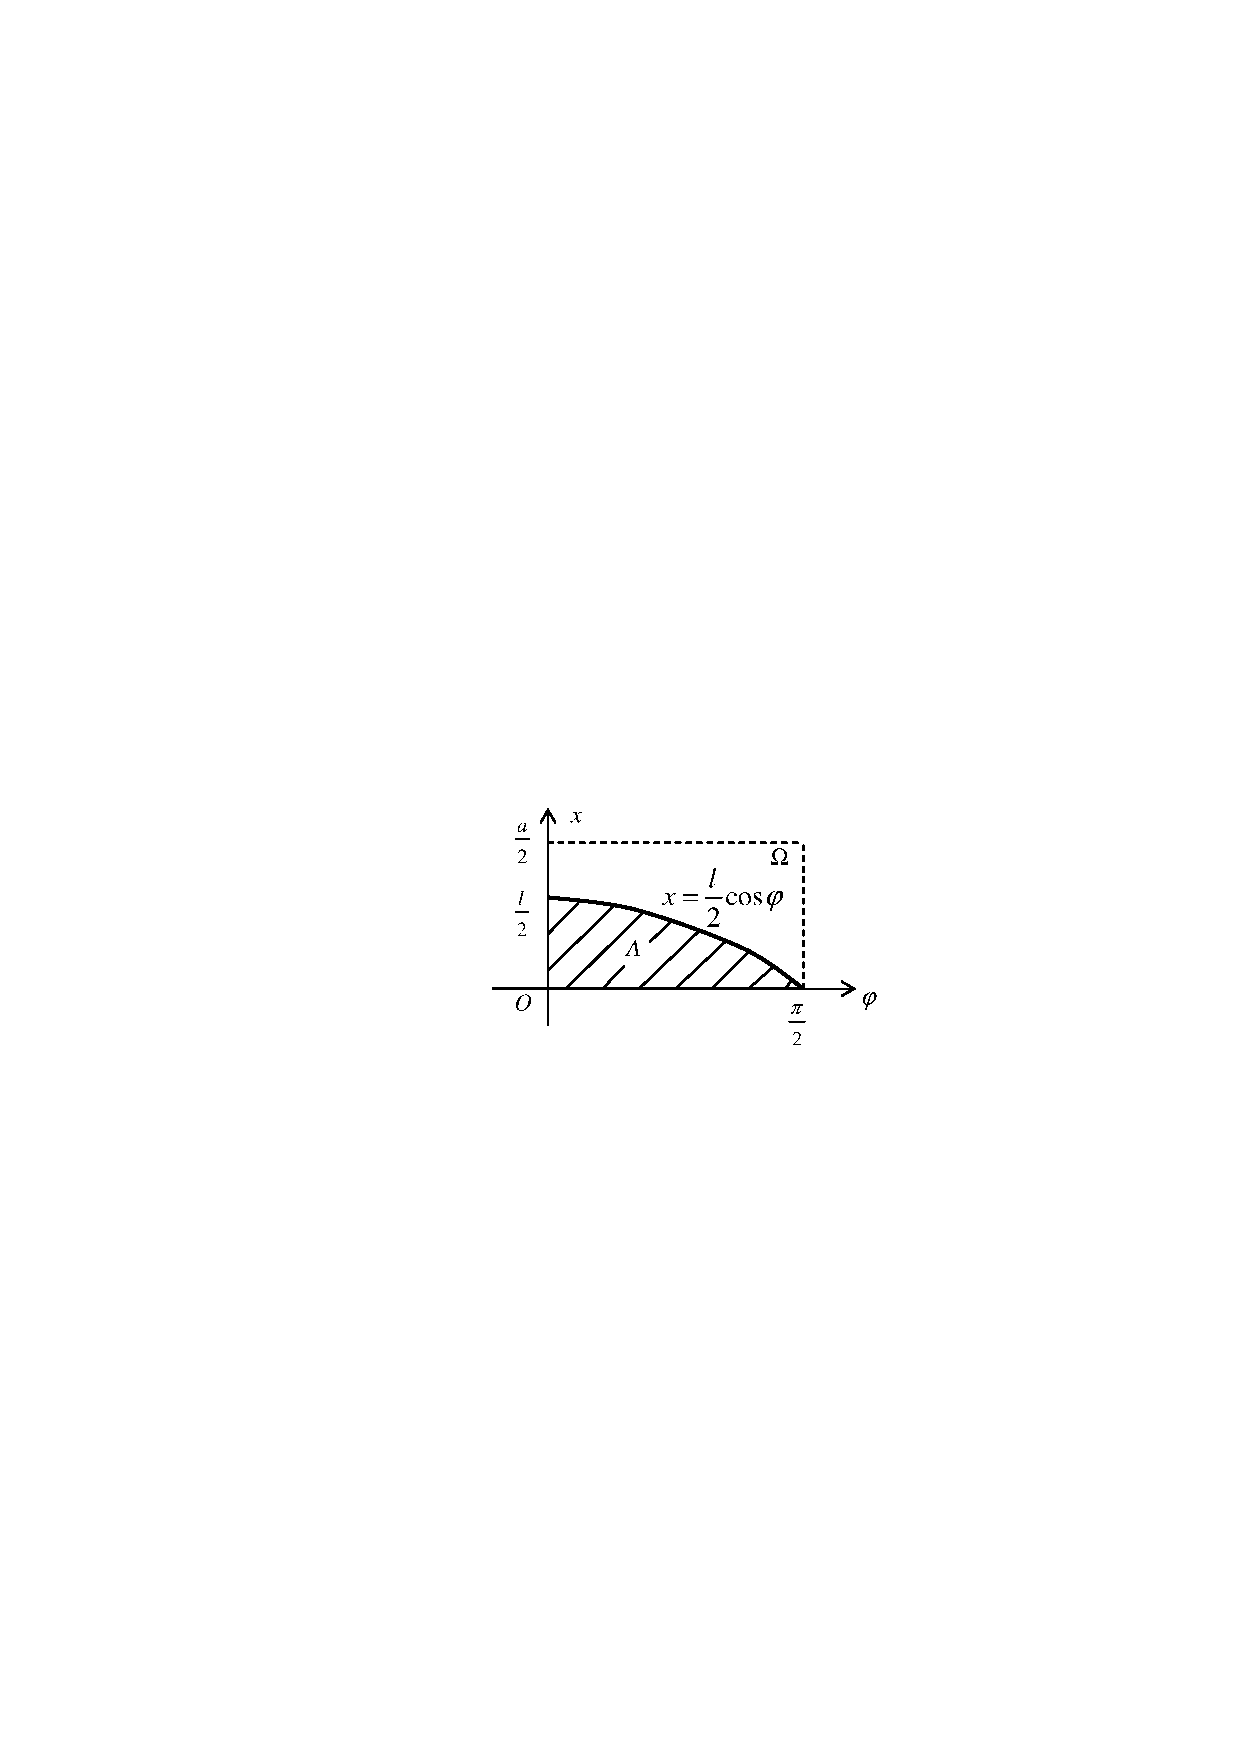
\includegraphics[]{pic/pic4}
	\caption{Пространство элементарных событий omega в задаче Бюффона}
	\label{fig4}
\end{figure}

\begin{example}[Задача Бюффона (1777 г.)]
	\label{ex:4.21}
На плоскости нарисовано счётное множество параллельных прямых. Расстояние между соседними прямыми равно $a$. На плоскость брошена игла длины $l < a$. Какова вероятность
того, что игла пересечёт одну из прямых?

\textit{Решение}. Возможные положения иглы на плоскости полностью определяются двумя координатами: расстоянием $x$ от середины иглы до ближайшей прямой и острым углом $\phi$ между иглой и перпендикуляром к параллельным прямым, см. рис. \ref{fig3}. Ясно, что $x \in [0, \frac{a}{2} ]$ и $\phi \in [0, \frac{\pi}{2} ]$. Поэтому множество $\Omega = [0, \frac{\pi}{2}] * [0, \frac{a}{2} ]$ есть пространство элементарных исходов этого эксперимента, см. рис. \ref{fig4}, и $\mu(\Omega) = \frac{\pi a}{4}$.

Событие $A =$\{игла пересечёт одну из прямых\} эквивалентно неравенству
$A = \{x \leq 2{{l}} \cos \phi \}$, поэтому множество благоприятных исходов располагается в пространстве $\Omega$ под графиком $x = \frac{ {{l}}}{2} \cos \phi$. Вычислим

$$\mu(A)=\int_{0}^{\frac{\pi}{2}} \frac{{{l}}}{2} \cos \phi d\phi = \frac{{{l}}}{2} \sin \phi \bigg|_0^{\frac{\pi}{2}} = \frac{{{l}}}{2}$$
Отсюда получаем $\P(A) = \frac{\mu(A)}{\mu(\Omega)}
 = \frac{2{{l}}}{\pi a}$
\end{example}
\begin{example}[<<Парадокс>> Бертрана\footnote{
	\label{ex:4.22}
	Жозеф Луи Франсуа Бертран (Joseph Louis Francois Bertrand, 1822 — 1900), французский математик.
}, 1888]
	
В круге наудачу выбирается хорда. Какова вероятность того, что её длина будет больше, чем длина стороны вписанного в круг правильного треугольника?

\textit{Решение}. Обозначим через $A$ событие, состоящее в том, что длина хорды будет больше, чем длина стороны вписанного в круг правильного треугольника. Существует по крайней мере три способа <<выбрать наудачу>> хорду в
круге.

\begin{figure}[H]
	\centering
	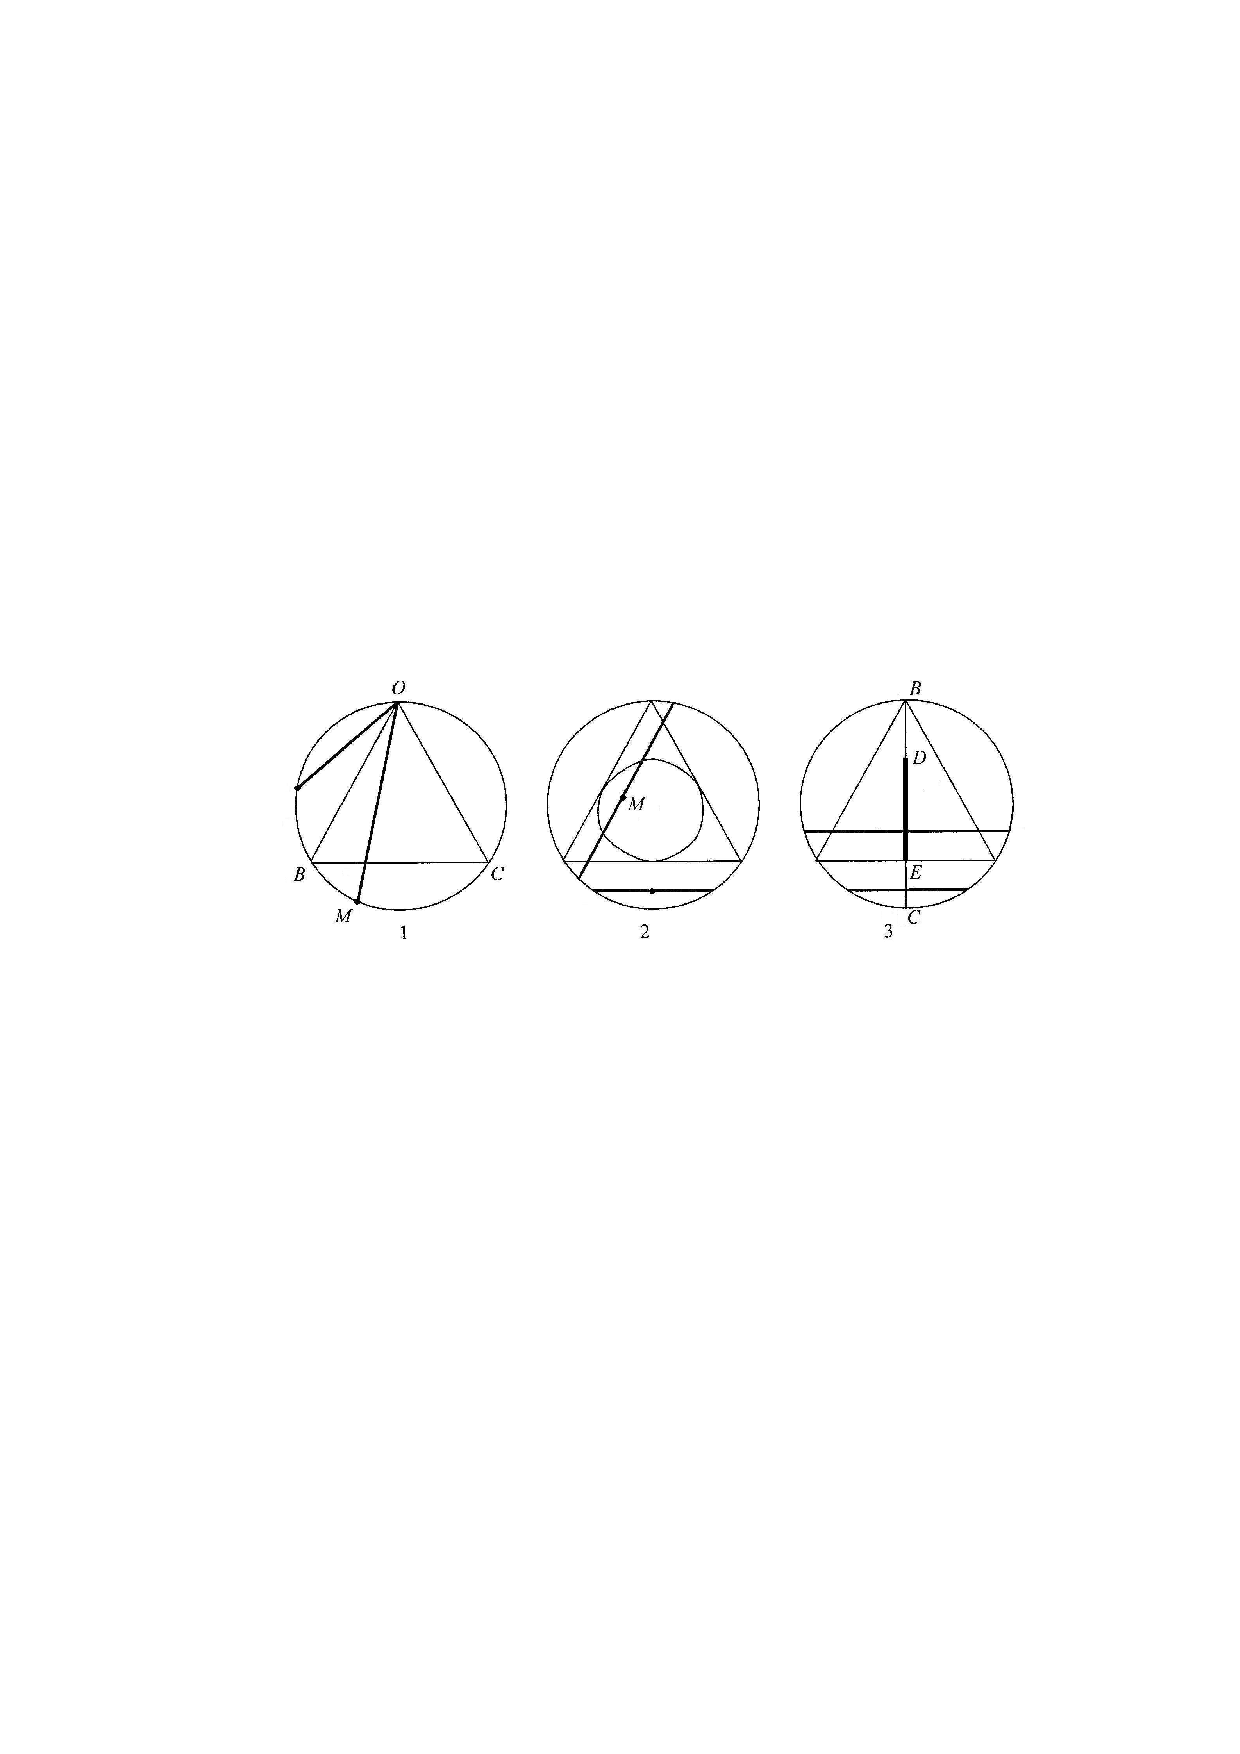
\includegraphics[]{pic/pic5}
	\caption{Парадокс Бертрана}
	\label{fig5}
\end{figure}

1-й способ. Зафиксируем один конец хорды $O$ на окружности. Положение другого конца хорды $M$ будем считать равномерно распределённым на окружности, см. рис. \ref{fig5}.1. Пусть координата конца $M$ хорды есть длина дуги $OM$ окружности, проходимой против часовой стрелки, тогда пространство элементарных событий $\Omega$ есть окружность, т.е. $\mu(\Omega) = 2 \pi R$. Благоприятным
исходом является положение конца хорды на дуге $BC$. Событие $A$ всех благоприятных исходов есть дуга $BC$, которая составляет третью часть окружности, т.е. $\mu(A) = \frac{2 \pi}{3} R$. Поэтому $\P(A) = \mu(\Omega) = \frac{1}{3}$.

2-й способ. Для каждой точки $M$ внутри круга (кроме его центра\footnote{
Т.к. вероятность попадания точки в центр круга равна нулю, то наступление этого события не влияет
на вероятность какого-либо события.
}) 
существует единственная хорда, для которой точка $M$ является её серединой, см. рис. \ref{fig5}.2. 

Поэтому, бросая точку $M$ в круг радиуса $R$, можно по ней однозначно восстановить хорду. Середину $M$ хорды будем считать равномерно распределённой в круге. Пространство элементарных событий $\Omega$ есть круг
радиуса $R$, его площадь $\mu(\Omega) = \pi R^2$. 

Благоприятными событию $A$ являются положения середины $M$ хорды внутри окружности, вписанной в треугольник. Легко подсчитать, что радиус вписанной окружности равен $\frac{R}{2}$ . Поэтому $\mu(A) = \frac{\pi R^2}{4}$ и $\P(A) = \frac{\mu(A)}{\mu(\Omega)} = \frac{1}{4}$.

3-й способ. Можно ограничиться рассмотрением только хорд, которые перпендикулярны какому-нибудь диаметру, например $C$ (остальные положения могут быть получены поворотом), см. рис. \ref{fig5}.3. 

Середину хорды будем считать равномерно распределённой на диаметре $BC$. Пространство элементарных событий omega есть диаметр $BC$, которому перпендикулярны хорды, его длина $\mu(\Omega) = 2R$. 

Благоприятными событию $A$ являются положения середины хорды на отрезке $DE$, лежащем на диаметре $BC$, так что центр отрезка $DE$ совпадает с центром круга. Можно видеть, что длина отрезка $DE$ есть $\mu(A) = R$. Поэтому $\P(A) = \frac{\mu(A)}{\mu(\Omega)} = \frac{1}{2}$.

Причина разных ответов заключается в том, что условие в круге наудачу выбирается хорда определяет эксперимент не однозначно. В решении мы провели три разных эксперимента по выбору хорды, и поэтому каждом случае был получен правильной ответ.

\end{example}

% \end{document}